% Options for packages loaded elsewhere
\PassOptionsToPackage{unicode}{hyperref}
\PassOptionsToPackage{hyphens}{url}
%
\documentclass[
]{article}
\usepackage{lmodern}
\usepackage{amssymb,amsmath}
\usepackage{ifxetex,ifluatex}
\ifnum 0\ifxetex 1\fi\ifluatex 1\fi=0 % if pdftex
  \usepackage[T1]{fontenc}
  \usepackage[utf8]{inputenc}
  \usepackage{textcomp} % provide euro and other symbols
\else % if luatex or xetex
  \usepackage{unicode-math}
  \defaultfontfeatures{Scale=MatchLowercase}
  \defaultfontfeatures[\rmfamily]{Ligatures=TeX,Scale=1}
\fi
% Use upquote if available, for straight quotes in verbatim environments
\IfFileExists{upquote.sty}{\usepackage{upquote}}{}
\IfFileExists{microtype.sty}{% use microtype if available
  \usepackage[]{microtype}
  \UseMicrotypeSet[protrusion]{basicmath} % disable protrusion for tt fonts
}{}
\makeatletter
\@ifundefined{KOMAClassName}{% if non-KOMA class
  \IfFileExists{parskip.sty}{%
    \usepackage{parskip}
  }{% else
    \setlength{\parindent}{0pt}
    \setlength{\parskip}{6pt plus 2pt minus 1pt}}
}{% if KOMA class
  \KOMAoptions{parskip=half}}
\makeatother
\usepackage{xcolor}
\IfFileExists{xurl.sty}{\usepackage{xurl}}{} % add URL line breaks if available
\IfFileExists{bookmark.sty}{\usepackage{bookmark}}{\usepackage{hyperref}}
\hypersetup{
  pdftitle={Employing co-expression networks to identify transcriptome diversification in maize lines},
  hidelinks,
  pdfcreator={LaTeX via pandoc}}
\urlstyle{same} % disable monospaced font for URLs
\usepackage{longtable,booktabs}
% Correct order of tables after \paragraph or \subparagraph
\usepackage{etoolbox}
\makeatletter
\patchcmd\longtable{\par}{\if@noskipsec\mbox{}\fi\par}{}{}
\makeatother
%Set text alignment and size
\usepackage{subfig}
\usepackage{titling}
\pretitle{\begin{flushleft}\Huge\textbf}
\posttitle{\par\end{flushleft}}
\preauthor{\begin{flushleft}\large}
\postauthor{\end{flushleft}}
\predate{\begin{flushleft}}
\postdate{\end{flushleft}}
%Set caption alignment
\usepackage[singlelinecheck=false,justification=justified]{caption}
% Allow footnotes in longtable head/foot
\IfFileExists{footnotehyper.sty}{\usepackage{footnotehyper}}{\usepackage{footnote}}
\makesavenoteenv{longtable}
\usepackage{graphicx}
\usepackage{float}
\makeatletter
\def\maxwidth{\ifdim\Gin@nat@width>\linewidth\linewidth\else\Gin@nat@width\fi}
\def\maxheight{\ifdim\Gin@nat@height>\textheight\textheight\else\Gin@nat@height\fi}
\makeatother
% Scale images if necessary, so that they will not overflow the page
% margins by default, and it is still possible to overwrite the defaults
% using explicit options in \includegraphics[width, height, ...]{}
\usepackage[a4paper, top=20mm, bottom=25mm, left=15mm, right=15mm]{geometry}
\setkeys{Gin}{width=\maxwidth,height=\maxheight,keepaspectratio}
% Set default figure placement to htbp
\makeatletter
\def\fps@figure{htbp}
\makeatother
\setlength{\emergencystretch}{3em} % prevent overfull lines
\providecommand{\tightlist}{%
  \setlength{\itemsep}{0pt}\setlength{\parskip}{0pt}}
\setcounter{secnumdepth}{-\maxdimen} % remove section numbering

\title{\protect\hypertarget{_heading=h.monioe1wkcaf}{}{}\textbf{Employing co-expression
networks to identify transcriptome diversification in maize lines}}

% Author contains Author and supervisor
\author{\textbf{Author:} Jan Izquierdo i Ramos\\
	\textbf{Scientific director:} Dr. Georg Haberer}%Author end

% Date contains date and Institutions (samll+italics for institutions)
\date{June 2025\\ %date
\small \textit{Plant Genome and Systems Biology, Environmental Health Center, Helmholtz Munich.\\ %Institutions
Address: Ingolstädter Landstraße 1, 85764 Neuherberg, Munich}
\footnotesize{Supplementary material and code available at GitHub: \href{https://github.com/Janek21/BDBI_TFG_MaizeCoexpression}{{https://github.com/Janek21/BDBI\_TFG\_MaizeCoexpression}}
}
}

\begin{document}
\maketitle

\hypertarget{abstract}{%
\section{Abstract}\label{abstract}}

Maize is one of the most important crops worldwide, valued for its high
yield potential, large genetic diversity, and remarkable adaptability.
The genetic diversity of maize has been extensively utilized in breeding
programs to enhance agronomic performance, and while this variability
has been well documented, its impact on transcriptional variation and
gene regulation across different lines remains mainly unexplored.

This study uses transcriptomic data from five maize lines---B73, DK150,
EP1, F7, and PE75---across 30 tissues, to provide a comprehensive
expression atlas for comparative analysis. The objective is to create
multi-line co-expression networks for examining gene co-expression
relationships simultaneously across different genotypes and tissues.

Through this approach, conserved and lineage-specific gene modules are
identified, offering insights into the transcriptional basis of
phenotypic similarities and differences among the maize lines studied.
Furthermore, the study uses these co-expression patterns to infer
functions for previously uncharacterized genes using the
guilt-by-association principle.

This study demonstrates that gene co-expression relationships exhibit
greater strength across distinct genetic lines compared to those
observed between different tissues within the same line, which
highlights potential regulatory relationships and divergent evolutionary
points. By mapping these tissue-line interactions, this study sets up a
foundation for deeper investigations into the regulatory mechanisms that
drive maize diversity and environmental adaptation as well as advancing
understanding on transcriptional networks and offering insights to
accelerate crop improvement initiatives.

\hypertarget{introduction}{%
\section{Introduction}\label{introduction}}

Maize is a widely produced crop, one of the 3 most important plants
worldwide, it surpasses the global production of wheat and rice and has
become a staple food around the world, it has uses as human and animal
aliment, as a resource in industrial products and as a model organism in
genetics. The widespread cultivation of this crop is because it presents
a high yield potential, extensive genetic diversity and is extremely
adaptable. The mentioned genetic diversity is manifested in the
existence of multiple maize germplasms like Flour maize, Sweet maize,
Dent maize and Flint maize. Also the use of this diversity has been
extensively exploited in breeding programs to increase agronomic
efficiency, the most common method is inter-group hybridization, which
exploits heterosis for better yields (Labroo et al., 2021).

This genetic diversity of maize has been well documented, pan-genome
studies present clear evidence of the multiple aspects that this crop
presents (Haberer et al., 2020). However, the effect of this high
genomic variability on the transcriptional variation of different maize
lines presents a lot of research opportunities. Understanding the
transcriptional diversity and differences present in these lines is
necessary for uncovering how genetic differences have affected the
regulation and functional pathways causing the phenotypic variations
into multiple maize lines. By analysing gene co-expression networks that
include multiple lines, relationships can be found between gene
expression, phenotypic traits and differences in genome structure and
organization.

To explore this, the present study focuses on five maize lines: B73,
DK150, EP1, F7 and PE75. B73 belongs to the U.S. Dent maize group and is
a widely used reference genotype, for example, it serves as a benchmark
for comparative analysis. DK150, EP1 and F7 are all European Flint
lines, originating from southern Germany, northern Spain and southern
France. And PE75 is a derivation from a German landrace, the Petkuser
Ferdinand Rot population, a doubled-haploid line to represent a more
genetically diverse background.

A comprehensive transcriptome atlas was generated to capture expression
profiles across 30 tissues in the 5 maize lines, with multiple samples
per tissue for a better representation of the data. This dataset will be
used for constructing a multi-genome co-expression network, enabling the
simultaneous comparison of the different tissues that belong to
different genotypes.

\hypertarget{gene-co-expression}{%
\subsection{Gene co-expression}\label{gene-co-expression}}

Gene co-expression typically employs pairwise comparisons of gene
expression levels, identifying genes that show similar expression
patterns across samples. As genes that exhibit correlated expression
patterns are often involved in the same biological processes, unknown
gene functions can be inferred based on the co-expression of genes with
known functions, this is known as the ``guilt-by-association''
principle.(Wolfe et al., 2005)

To quantify co-expression correlation measures are used, among these
measures Pearson and Spearman correlations stand out as the most common,
Spearman presents no distributional assumptions while Pearson assumes
normally distributed data, this makes Spearman more robust in settings
that present heterogeneous samples or nonlinear regulatory mechanisms,
which is not the case of this study.

Gene co-expression is a first step in developing co-expression
networks(Figure 1), which provide understanding among whole sets of
genes and allow for much more confidence in the identification of
functional gene modules, regulatory pathways and key genes in biological
processes. This is because of the capacity to identify clusters of
tightly related genes which are likely to share common biological
functions, this causes that the functions of unknown genes in a cluster
can be inferred by the ``guilt-by-association'' principle when in the
same cluster as well-characterized genes.
 

\begin{figure}[H]
	\centering
	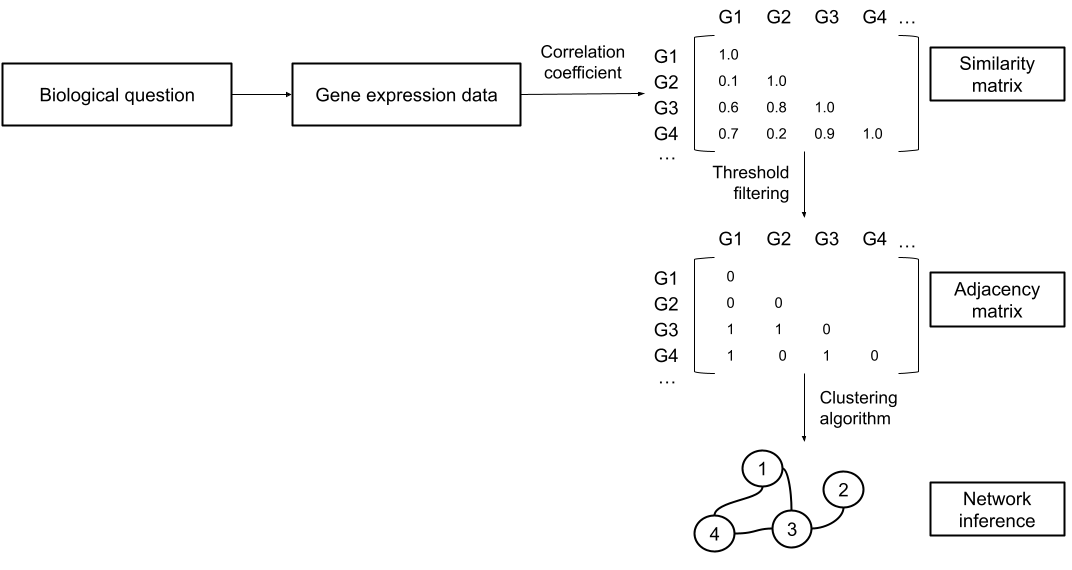
\includegraphics[width=1\linewidth]{figures/Final_networkProcess.png}
	\caption[Network Diagram]{\small Simplified representation of the process for network building.(Serin et al., 2016, p. 4)}
	\label{fig:Netw_diagram}
\end{figure}

By constructing co-expression networks across five distinct maize lines
and 30 different tissues this study seeks to improve our understanding
of how gene co-expression reflects underlying genomic differences,
ultimately providing new insights into the regulatory features that
drive maize diversity and adaptation.

\hypertarget{objectives}{%
\section{Objectives}\label{objectives}}

This study intends to understand the relationship between the gene
expression patterns in 5 different maize lines and the phenotypic
differences they present by the employment of gene co-expression
networks.

An essential part of the study is to determine whether common gene
modules are present across the maize lines, how they relate to
phenotypic similarities, which functions tend to be present in the
modules and the relation between the presence of these functions and the
traits to which these modules relate to. Complementary to this
objective, the study also aims to examine the diverging modules across
lines, the contribution of the possible transcriptional variations to
phenotypic divergence and to discover functional annotation of unknown
genes.

The ultimate goal of this research is to contribute to a broader
understanding of the maize transcriptome by offering insights into the
effect that gene expression has on genetic diversity. The finality that
it leads to is to provide a basis for further research on maize
breeding, genetic adaptation, and crop improvement.

\hypertarget{methodology}{%
\section{Methodology}\label{methodology}}

The following explanation provides an overview of the processes involved
in the preparation of the data, creation of the network and function
analysis.

\hypertarget{data-filtering}{%
\subsection{Data filtering}\label{data-filtering}}

The data is cleaned from errors and low quality samples are filtered
out. The high quality samples are identified by belonging to the quality
0 group in the metadata, also, discrepancies between the number of data
and metadata samples were found and corrected by eliminating pollen
tissue samples, which are present as metadata but present no expression
data, as not enough genetic material could be extracted for successful
sequencing.

\hypertarget{replicates-in-the-data}{%
\subsection{Replicates in the data}\label{replicates-in-the-data}}

The first step involved detecting and removing outlier genes, data
points which would heavily skew the data while contributing minimally to
biological relevance. The metadata was expanded to include the tissue
and line data on the same instance, which was needed for merging the
tissue data of each genotype to address potential imbalances and a high
dimensionality. This merging process equalizes the discrepancies caused
by differences in replicate numbers, which also skew results, and it is
done through calculating the mean of the replicates for that genotype
and tissue.

\hypertarget{normalization}{%
\subsection{Normalization}\label{normalization}}

The goal of normalization is to ensure that read counts represent
differences in true gene expression, enabling meaningful comparisons
across samples and reducing noise in the data.

In this study, normalization was performed by library size, more
concretely using the Reads Per Kilobase per Million mapped reads (RPKM),
although Counts Per Million (CPM) is also a valid alternative, it was
not used due to a better resolution after filtering when using RPKM. The
program hinges on the edgeR R package to provide the normalization and
it uses the same process to apply a logarithmic transformation to the
data. After normalization the data presented an overrepresentation of
lowly expressed genes, so to improve the quality of the normalized data,
the lowly expressed genes were removed through gene expression
filtering, which enhances Differentially Expressed Genes (DEG)
detection.

The applied filtering strategy preserves genes if they present at least
one value greater or equal than 0 (at least 1 count for the gene across
all replicates), this is to keep the maximum number of possibly
correlated patterns as possible, while disregarding the genes that
present the least expression.

\begin{figure}[H]
	\centering
	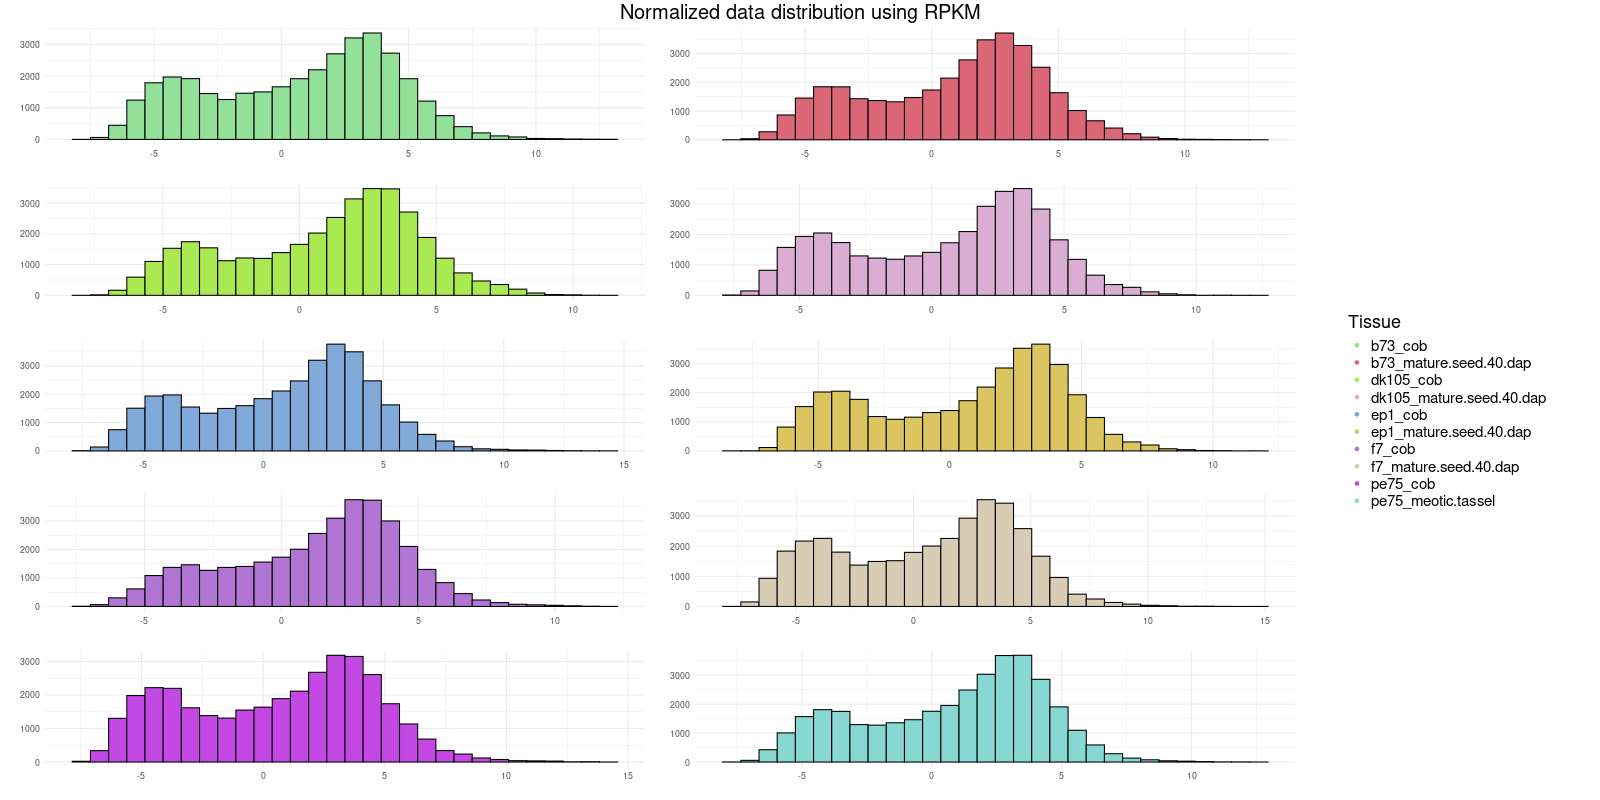
\includegraphics[width=1\linewidth]{figures/normRPKM_distPlot.png}
	\caption[RPKM distribution]{\small RPKM distribution filtered by expression for 2 tissues of each line. The data fits a bimodal distribution for all of the analyzed tissues, so it can be safely assumed that the bimodal distribution is applicable to all tissues. PE75 presents no samples for mature seed 40, so meiotic tassel is used in the display.}
	\label{fig:}
\end{figure}

\hypertarget{expression-data-analysis}{%
\subsection{Expression data analysis}\label{expression-data-analysis}}

For a better comprehension of the data and to grasp at possible
correlations within the data, PCA and UMAP analysis were performed.
These allow for the visualization of expression patterns in the data and
to glimpse into underlying correlations between lines and tissues.

\includegraphics[width=6.69272in,height=3.34722in]{media/image11.png}\emph{Figure
3: Representations of gene expression with features according to tissues
and lines. The representation is a UMAP where clusters by expression
similarity can be observed.}

In Figure 3 it can be observed that co expression relations tend to be
stronger for tissue than for line, as an example, leaf blades of
multiple tissues cluster together rather than clustering with leaf
seathes or leaf meristems of the same line, therefore it can be assumed
that in the creation of the network the tissues will present strong
correlation within a module. More examples can be observed, as is the
case of the seed groups.

These exploratory expression data analysis allow for a better knowledge
of patterns to search for later in the analysis.

\hypertarget{network-construction-and-gene-clustering}{%
\subsection{Network construction and gene
clustering}\label{network-construction-and-gene-clustering}}

The next step in constructing the gene co-expression network involves
clustering genes while maintaining an appropriate soft-thresholding
power. To determine the appropriate power for each case, the program
considers the signed R\textsuperscript{2} and the mean connectivity,
selecting the optimal value from a range of 1 to 17 and odd numbers
between 17 and 49. The value is limited to 30, as that is the maximum
soft power allowed for clustering.

The gene clustering process is performed by a WGCNA(Langfelder \&
Horvath, 2008) function that has its parameters set to allow for a
single-block approach and which uses hierarchical clustering methods.
The factors that have the most influence on this clustering are the
initial normalization and filtering methods, the function parameters and
the soft-thresholding power selection, as it impacts the overall network
structure. The effects can be seen in the amount of modules in which
genes are classified into, and consequently, the amount of genes present
in each module. In the case of our study 39 modules were revealed, with
sizes between 28(\emph{plum1)} and 4926\emph{(turquoise}) and a mean
size of 914 genes. The grey module, which generally contains the worst
clustered genes, contained only 11.2\% of the total, indicating a
successful module separation, even though it could be refined further.

From the creation of this network, the principal components of each
module's expression matrices are collected together in an adjacency
table with a binary matrix of replicate relationships. This adjacency
table is the object utilized to calculate the correlations between the
gene modules and replicates, and enables the downstream analysis of
module-trait relationships, so that cross-genotype and cross-tissue
modules may be identified.

\hypertarget{function-significance-in-modules}{%
\subsection{Function significance in
modules}\label{function-significance-in-modules}}

The data from the tables presents multiple expression groupings by lines
and tissues, to analyze the biological significance of each module, the
functions of the genes that form each of these blocks has to be
analyzed. For this analysis a table showing the genes associated with
each module is written from the previous computation.

For obtaining the functional gene annotations of the genes in the maize
lines mercator4 was used with the Zea Mays B73 data as a base, this
generated a file containing the functional annotation for the gene as
well as the swissprot, prot-scriber and mercator protein annotations.

To be able to classify these functionally annotated genes to their
corresponding modules, a python program counts all the repetitions of
each function in all modules and in each individual module and uses this
data to perform a Fisher test and prove significance of the different
functions in each module.

The program has to filter out all unannotated entries and all entries
that belong to Enzyme functions, as those are molecular functions and
the focus of the analysis lies on biological functions, therefore they
are of no interest and are removed from the universe of the statistical
test.

The enriched modules presented different significance levels for
distinct biological functions, as can be seen in Figure 4, which is a
summary table that lists the most significant functions of all modules.

\begin{longtable}[]{@{}lll@{}}
\toprule
\emph{Function} & \emph{Pvalue} & \emph{Module}\tabularnewline
\midrule
\endhead
Vesicle trafficking & 6.52023951744159E-148 & salmon\tabularnewline
Chromatin organisation & 2.2479313916297E-108 & red\tabularnewline
Photosynthesis & 0 & turquoise\tabularnewline
Cellular respiration & 8.20718680827369E-148 &
paleturquoise\tabularnewline
Protein biosynthesis & 1.84219326457758E-41 & yellow\tabularnewline
Cell wall organisation & 1.04670469138908E-48 & yellow\tabularnewline
Cell division & 1.63419134542279E-55 & lightcyan\tabularnewline
Protein biosynthesis & 3.95106070433327E-42 & grey\tabularnewline
Cell division & 5.97864496091729E-60 & blue\tabularnewline
Protein biosynthesis & 1.23671252432881E-249 & blue\tabularnewline
\bottomrule
\end{longtable}

Figure 4: Table illustrating the 10 most significant functions across
all modules

\hypertarget{gene-function-analysis}{%
\subsection{Gene function analysis}\label{gene-function-analysis}}

After looking into the composition of the modules and the functions that
each of them performed, a deeper analysis was in order to comprehend the
modules at gene level. The goal of this analysis was to search for gene
functions on a smaller level than modules and to uncover functions of
unknown genes, as a gene by gene inspection provides the ability to
target more concrete groups and individual genes for more specific
analysis of relations and functions.

This process was done at module level, isolating the genes belonging to
a particular module from the RNA-seq data and holding them to the same
processes used previously on the whole data, meaning that they were
joined by tissue and RPKM normalized. A correlation table was computed
using this data and the genes were clustered according to the
co-expression computations. The first algorithm by which the genes were
processed was the K-means clustering, as it is a flexible, efficient and
easy to implement method. The algorithm uses a number of centroids
optimized by sum of squares, but this clustering method was abandoned as
the clustering was of a too coarse grain, not offering enough
distinction and biological significance. The alternative method that was
chosen for computing the gene clustering was a Louvain community
clustering, which allows for an improved resolution and biological
significance(Figure 5) as communities work on building clusters based on
closely correlated nodes instead of closeness to a centroid as K-means
does. For this type of clustering a threshold has to be chosen, this
threshold represents the cutoff point of correlation between the genes
and it determines the amount of genes and the number of communities, the
threshold optimization for each module was done manually.

From the communities the GO functions for each gene are obtained, which
allows to unveil unannotated genes and to use the
``guilt-by-association'' rule to assign functions based on the ones
present in closely related genes. To do this the process was to take the
genes in the Louvain communities, and obtain the GO terms related to
these genes and the functions corresponding to the GO terms, the unknown
genes were determined by being the ones that presented no GO term
associations. Then the functions of all highly correlated genes(to the
unknown genes) were obtained, and filtered by significance, keeping only
the 10 most significant functions. By using the ``guilt-by-association''
rule it is possible to determine that the unannotated genes will present
these functions.

\includegraphics[width=7.00104in,height=3.58143in]{media/image12.png}

Figure 5: Representation of Louvain communities in the central node of
correlations for the turquoise module when using a 0.6 threshold.

\hypertarget{results-and-discussion}{%
\section{Results and discussion}\label{results-and-discussion}}

\hypertarget{correlations}{%
\subsection{Correlations}\label{correlations}}

The co-expression analysis produces a correlation table which contains
the gene expression grouped by modules and the traits from all lines
that are to be analyzed.

\includegraphics[width=6.69272in,height=3.34722in]{media/image6.png}

\emph{Figure 6: Correlation plot with the x axis sorted by lines,
groupings by correlation according to the line which the tissue belongs
to can be observed, representing feature similarities between the lines.
The y axis represents groupings of genes by expression pattern
similarity.}

In Figure 6, it can be observed that there are gene modules that
manifest in blocks by lines, some are expressed in multiple lines while
some are expressed only in one, for example, module \emph{darkturquoise}
is overexpressed in EP1, F7 and PE75 while \emph{magenta} is only is
expressed in B73. These clusters of expression for each module represent
similar expression patterns, which means the lines are closely related.
When lines are expressed exclusively in a module, then it can also be
deduced that the module performs functions that identify these lines
from the rest.

These differences present biological significance, for example, most
modules present in B73 are not present in any of the other lines, this
is because of a germplasm and location difference, B73 is a U.S. dent
line while the other lines belong to European flint.

\includegraphics[width=6.69272in,height=3.34722in]{media/image5.png}

\emph{Figure 7: Correlation plot with the x axis sorted according to
tissues, strong correlation among tissues of different lines can be
spotted, representing similar gene functions in certain tissues. The y
axis represents groupings of genes by expression pattern similarity.}

Apart from the modules clustered by genotype, there are more modules
that appear scattered, to observe if they formed patterns by tissue, the
correlation graph was ordered accordingly. The resulting plot can be
observed in Figure 7 in which groups, different than in the ones present
in Figure 6, can also be identified, these groups form patterns around
different tissues, and the patterns repeat around one or more modules,
creating clusters of expression for various modules and tissues. For
example, the \emph{violet} and \emph{black} modules present strong
correlations for all immature and meiotic tassels and the
\emph{turquoise} module strongly correlates leaf tissues, both of these
cases, the tissue groupings follow the earlier observations (Figure 3),
it is the case with most tissues, and can be used to corroborate the
results.

These clusters by tissue indicate expression similarities across
genotypes, where the function of the tissue is more impactful in
expression than the line to which it belongs.

\hypertarget{module-functions}{%
\subsection{Module functions}\label{module-functions}}

All functional modules are groups of genes, therefore by analyzing the
composition of the modules their main functions can be identified.
Hypotheses can be made for module functions based on the tissues in
which there is a strong correlation, as an example, the \emph{turquoise}
module is mainly represented in leaf tissues, so the main functions it
will present are probably related to photosynthesis, the \emph{black}
and \emph{violet} modules present strong correlations with immature and
meiotic tassels, which develop male flower structure and form pollen, so
the main functions it will present are most likely related to the
creation of new structures and plant reproduction and the
\emph{yellowgreen}, \emph{blue} and \emph{darkgreen} modules can be
observed with strong correlations in immature cob, prepollinated cob and
seeds, which means that the genes in this modules are mainly in charge
of synthesis and cell division.

\includegraphics[width=6.69272in,height=3.34722in]{media/image3.png}

\emph{Figure 8: Graph provided for the visualization of significant
functions per module, it allows for a clear association in the functions
performed by each module and therefore by the tissues associated to that
module as well.}

In Figure 8 the significant functions in each module can be observed,
and the functions of highest significance are highlighted, which can be
used for corroborating hypotheses like the previous one. It can be
observed that the photosynthesis function is of strong significance in
the \emph{turquoise} module and that reproductive functions, like plant
reproduction and cell division, as well as structural functions, like
protein synthesis and cell wall organization, are significant in the
\emph{black} and \emph{violet} modules. It can also be observed that the
\emph{yellowgreen}, \emph{blue} and \emph{darkgreen} modules not only
present high significance for cell division, protein synthesis and RNA
synthesis but also for other functions like solute transport and
photosynthesis.

The inspections into the functions of individual modules can also be
used to discover more about differences of function execution in lines,
that being in exclusivity to a line or execution similarities between 2
or more lines. In the correlation plots (Figure 6) it can be observed
that there are modules which present exclusive coexpression relations
within a line, like module \emph{magenta}, which is only expressed in
B73 and presents strong significance for functions like DNA damage
response or protein and RNA homeostasis, indicating that this line
performs the functions via a different genes than other lines.

\hypertarget{individual-gene-analysis}{%
\subsection{Individual gene analysis}\label{individual-gene-analysis}}

After the analysis of the modules, a deeper analysis was in order, as
from the module functions a general functional knowledge is obtained,
but an individual gene analysis allows for specification and targeting
in the inspections, even when the modules present unknown genes, as the
functions of these can be identified using co-expression methods.

The functions for the communities should be closely related to the
module functions, but distilled to a finer grain. Hypotheses can be made
as to the functions present in the communities, as an example, in the
\emph{turquoise} module which presents photosynthetic functions, the
gene functions in the communities will mainly be metabolic processes,
like calvin cycle regulation and other synthesization functions.
Communities present unknown genes (Figure 9) , which can be associated
with the functions present in the community using the
``guilt-by-association'' rule; these associations provide a better
understanding of the communities as a whole as well as the ability to be
used in the case of a need for more detail in an unknown gene.

\includegraphics[width=6.69272in,height=4.01389in]{media/image14.png}

\emph{Figure 9: This figure represents a community of the turquoise
module, the unknown genes are marked in black while the known genes are
blue. It can be observed that there is a very high proportion of unknown
genes, which translates into a low confidence level in the significant
functions.}

For concrete function identification in the unknown genes a table
similar to the one seen in Figure 10 can be consulted, it provides a
better insight into the functions by association assigned to each of the
unknown genes. This table is key in understanding functions in fine
grain on each module, as functions at community and gene level are able
to be consulted

\begin{longtable}[]{@{}llll@{}}
\toprule
\emph{Community} & \emph{Unknown} & \emph{Annotated} &
\emph{Function}\tabularnewline
\midrule
\endhead
\begin{minipage}[t]{0.22\columnwidth}\raggedright
C16\strut
\end{minipage} & \begin{minipage}[t]{0.22\columnwidth}\raggedright
Zm00001eb215370\strut
\end{minipage} & \begin{minipage}[t]{0.22\columnwidth}\raggedright
Zm00001eb118870

Zm00001eb054390\strut
\end{minipage} & \begin{minipage}[t]{0.22\columnwidth}\raggedright
\strut
\end{minipage}\tabularnewline
\begin{minipage}[t]{0.22\columnwidth}\raggedright
C16\strut
\end{minipage} & \begin{minipage}[t]{0.22\columnwidth}\raggedright
Zm00001eb085230\strut
\end{minipage} & \begin{minipage}[t]{0.22\columnwidth}\raggedright
Zm00001eb146130

Zm00001eb107670

Zm00001eb121270

Zm00001eb077770

Zm00001eb367960

Zm00001eb299510\strut
\end{minipage} & \begin{minipage}[t]{0.22\columnwidth}\raggedright
plant-type cell wall organization

plant-type cell wall organization or biogenesis

binding

cell wall organization

cell growth

external encapsulating structure organization

regulation of cell size

developmental process

growth

cell wall organization or biogenesis\strut
\end{minipage}\tabularnewline
\begin{minipage}[t]{0.22\columnwidth}\raggedright
C16\strut
\end{minipage} & \begin{minipage}[t]{0.22\columnwidth}\raggedright
Zm00001eb061350\strut
\end{minipage} & \begin{minipage}[t]{0.22\columnwidth}\raggedright
Zm00001eb192560

Zm00001eb067980

Zm00001eb018090

Zm00001eb357050\strut
\end{minipage} & \begin{minipage}[t]{0.22\columnwidth}\raggedright
\strut
\end{minipage}\tabularnewline
C16 & Zm00001eb265640 & Known & \vtop{\hbox{\strut plastid
transcription}\hbox{\strut transferase activity}\hbox{\strut regulation
of cellular process}\hbox{\strut chloroplast thylakoid
membrane}\hbox{\strut thylakoid membrane
organization}\hbox{\strut seedling
development.membrane}\hbox{\strut deoxyribodipyrimidine photo-lyase
activity}\hbox{\strut chloroplast relocation}}\tabularnewline
\begin{minipage}[t]{0.22\columnwidth}\raggedright
C16\strut
\end{minipage} & \begin{minipage}[t]{0.22\columnwidth}\raggedright
Zm00001eb284770\strut
\end{minipage} & \begin{minipage}[t]{0.22\columnwidth}\raggedright
Zm00001eb116580

Zm00001eb373490

Zm00001eb225060

Zm00001eb264880

Zm00001eb087570

Zm00001eb413170\strut
\end{minipage} & \begin{minipage}[t]{0.22\columnwidth}\raggedright
lipid biosynthetic process

catalytic activity

lipid metabolic process

primary metabolic process

metabolic process

cellular process

biological\_process

cellular anatomical structure

cellular\_component

molecular\_function\strut
\end{minipage}\tabularnewline
C16 & Zm00001eb164890 & Zm00001eb164880 &\tabularnewline
\bottomrule
\end{longtable}

\emph{Figure 10: Representation of a sample of genes belonging to
community 16 in the turquoise module, genes can be observed presenting
no associated functions, this is mainly due to a lack of significance
for any functions the closely correlated genes present}

\hypertarget{conclusion}{%
\section{Conclusion}\label{conclusion}}

This study has examined multiple maize transcriptomes with the aim of
uncovering patterns for a deeper understanding of the diversification
across maize lines, which would contribute to an overall deeper
understanding of maize genetics. While no single conclusion was sought
the analysis has provided insights into important aspects of maize gene
expression and its workings across various lines.

In this study, several sections in the transcriptomes have been
identified as being closely correlated across the lines, which indicates
points of similarity; these points of similarity are tissues where the
genes present in these lines perform very similar functions. These
findings highlight potential regulatory relationships and divergent
evolutionary points, which motivates further investigation through
functional validation and targeted studies to confirm and improve these
findings.

The study also provides a more detailed analysis of the functions shared
across the lines and tissues, allowing to determine that genes often
present higher correlation in particular tissues across different lines
than with other tissues within their own line. This points to these
genes executing specialized functions in the particular tissues, like
reproductive functions for tassel tissue or photosynthetic functions for
leaf tissue, hypotheses which are proved to be true by analyzing groups
of genes, the tissues in which they are mainly expressed and the
functions which they perform.

Even though these analyses provide large amounts of data for further
research the specification of the data can yet be taken a step further.
By an analysis of particular genes and the functions they perform, very
specialized and concrete evaluations can be made. The issue arises as
many of these genes present unknown functional annotations, but to
circumvent this, the steps have been taken to associate functions to
genes according to the ``guilt-by-association'' rule, producing a frame
of reference where the concrete, specialized analysis can truly be
sought for any particular gene of interest.

Overall the study has produced a broad range of results, however the
analysis only contemplates the surface potential of the data. Further
studies on the produced information could reach a higher understanding
of the steps of diversification in maize and of the effect of shared
features and relations between lines.

\hypertarget{bibliography}{%
\section{Bibliography}\label{bibliography}}

Beiki, H., Nejati-Javaremi, A., Pakdel, A., Masoudi-Nejad, A., Hu,
Z.-L., \& Reecy, J. M. (2016). Large-scale gene co-expression network as
a source of functional annotation for cattle genes. BMC Genomics, 17(1),
846.
\href{https://doi.org/10.1186/s12864-016-3176-2}{{https://doi.org/10.1186/s12864-016-3176-2}}

Chang, Y.-M., Lin, H.-H., Liu, W.-Y., Yu, C.-P., Chen, H.-J., Wartini,
P. P., Kao, Y.-Y., Wu, Y.-H., Lin, J.-J., Lu, M.-Y. J., Tu, S.-L., Wu,
S.-H., Shiu, S.-H., Ku, M. S. B., \& Li, W.-H. (2019). Comparative
transcriptomics method to infer gene coexpression networks and its
applications to maize and rice leaf transcriptomes. Proceedings of the
National Academy of Sciences, 116(8), 3091--3099.
\href{https://doi.org/10.1073/pnas.1817621116}{{https://doi.org/10.1073/pnas.1817621116}}

Childs, K. L., Davidson, R. M., \& Buell, C. R. (2011). Gene
Coexpression Network Analysis as a Source of Functional Annotation for
Rice Genes. PLOS ONE, 6(7), e22196.
\href{https://doi.org/10.1371/journal.pone.0022196}{{https://doi.org/10.1371/journal.pone.0022196}}

de Silva, K. K., Dunwell, J. M., \& Wickramasuriya, A. M. (2022).
Weighted Gene Correlation Network Analysis (WGCNA) of Arabidopsis
Somatic Embryogenesis (SE) and Identification of Key Gene Modules to
Uncover SE-Associated Hub Genes. International Journal of Genomics,
2022(1), 7471063.
\href{https://doi.org/10.1155/2022/7471063}{{https://doi.org/10.1155/2022/7471063}}

Downs, G. S., Bi, Y.-M., Colasanti, J., Wu, W., Chen, X., Zhu, T.,
Rothstein, S. J., \& Lukens, L. N. (2013). A developmental
transcriptional network for maize defines coexpression modules. Plant
Physiology, 161(4), 1830--1843.
\href{https://doi.org/10.1104/pp.112.213231}{{https://doi.org/10.1104/pp.112.213231}}

Evans, C., Hardin, J., \& Stoebel, D. M. (2017). Selecting
between-sample RNA-Seq normalization methods from the perspective of
their assumptions. Briefings in Bioinformatics, 19(5), 776--792.
\href{https://doi.org/10.1093/bib/bbx008}{{https://doi.org/10.1093/bib/bbx008}}

Grote, U., Fasse, A., Nguyen, T. T., \& Erenstein, O. (2021). Food
Security and the Dynamics of Wheat and Maize Value Chains in Africa and
Asia. Frontiers in Sustainable Food Systems, 4.
\href{https://doi.org/10.3389/fsufs.2020.617009}{{https://doi.org/10.3389/fsufs.2020.617009}}

Guo, W., Schreiber, M., Marosi, V. B., Bagnaresi, P., Jørgensen, M. E.,
Braune, K. B., Chalmers, K., Chapman, B., Dang, V., Dockter, C., Fiebig,
A., Fincher, G. B., Fricano, A., Fuller, J., Haaning, A., Haberer, G.,
Himmelbach, A., Jayakodi, M., Jia, Y., \ldots{} Waugh, R. (2025). A
barley pan-transcriptome reveals layers of genotype-dependent
transcriptional complexity. Nature Genetics, 57(2), 441--450.
\href{https://doi.org/10.1038/s41588-024-02069-y}{{https://doi.org/10.1038/s41588-024-02069-y}}

Haberer, G., Kamal, N., Bauer, E., Gundlach, H., Fischer, I., Seidel, M.
A., Spannagl, M., Marcon, C., Ruban, A., Urbany, C., Nemri, A.,
Hochholdinger, F., Ouzunova, M., Houben, A., Schön, C.-C., \& Mayer, K.
F. X. (2020). European maize genomes highlight intraspecies variation in
repeat and gene content. Nature Genetics, 52(9), 950--957.
\href{https://doi.org/10.1038/s41588-020-0671-9}{{https://doi.org/10.1038/s41588-020-0671-9}}

Han, L., Zhong, W., Qian, J., Jin, M., Tian, P., Zhu, W., Zhang, H.,
Sun, Y., Feng, J.-W., Liu, X., Chen, G., Farid, B., Li, R., Xiong, Z.,
Tian, Z., Li, J., Luo, Z., Du, D., Chen, S., \ldots{} Li, L. (2023). A
multi-omics integrative network map of maize. Nature Genetics, 55(1),
144--153.
\href{https://doi.org/10.1038/s41588-022-01262-1}{{https://doi.org/10.1038/s41588-022-01262-1}}

Huang, J., Vendramin, S., Shi, L., \& McGinnis, K. M. (2017).
Construction and Optimization of a Large Gene Coexpression Network in
Maize Using RNA-Seq Data. Plant Physiology, 175(1), 568--583.
\href{https://doi.org/10.1104/pp.17.00825}{{https://doi.org/10.1104/pp.17.00825}}

Kitano, H. (2004). Biological robustness. Nature Reviews Genetics,
5(11), 826--837.
\href{https://doi.org/10.1038/nrg1471}{{https://doi.org/10.1038/nrg1471}}

Labroo, M. R., Studer, A. J., \& Rutkoski, J. E. (2021). Heterosis and
Hybrid Crop Breeding: A Multidisciplinary Review. Frontiers in Genetics,
12, 643761.
\href{https://doi.org/10.3389/fgene.2021.643761}{{https://doi.org/10.3389/fgene.2021.643761}}

Langfelder, P., \& Horvath, S. (2008). WGCNA: An R package for weighted
correlation network analysis. BMC Bioinformatics, 9(1), 559.
\href{https://doi.org/10.1186/1471-2105-9-559}{{https://doi.org/10.1186/1471-2105-9-559}}

Mayer, M., Hölker, A. C., Presterl, T., Ouzunova, M., Melchinger, A. E.,
\& Schön, C.-C. (2022). Genetic diversity of European maize landraces:
Dataset on the molecular and phenotypic variation of derived
doubled-haploid populations. Data in Brief, 42, 108164.
\href{https://doi.org/10.1016/j.dib.2022.108164}{{https://doi.org/10.1016/j.dib.2022.108164}}

Ranum, P., Peña-Rosas, J. P., \& Garcia-Casal, M. N. (2014). Global
maize production, utilization, and consumption. Annals of the New York
Academy of Sciences, 1312(1), 105--112.
\href{https://doi.org/10.1111/nyas.12396}{{https://doi.org/10.1111/nyas.12396}}

Serin, E. A. R., Nijveen, H., Hilhorst, H. W. M., \& Ligterink, W.
(2016). Learning from Co-expression Networks: Possibilities and
Challenges. Frontiers in Plant Science, 7.
\href{https://doi.org/10.3389/fpls.2016.00444}{{https://doi.org/10.3389/fpls.2016.00444}}

Sha, Y., Phan, J. H., \& Wang, M. D. (2015). Effect of low-expression
gene filtering on detection of differentially expressed genes in RNA-seq
data. Annual International Conference of the IEEE Engineering in
Medicine and Biology Society. IEEE Engineering in Medicine and Biology
Society. Annual International Conference, 2015, 6461--6464.
\href{https://doi.org/10.1109/EMBC.2015.7319872}{{https://doi.org/10.1109/EMBC.2015.7319872}}

Stuart, J. M., Segal, E., Koller, D., \& Kim, S. K. (2003). A
Gene-Coexpression Network for Global Discovery of Conserved Genetic
Modules. Science, 302(5643), 249--255.
\href{https://doi.org/10.1126/science.1087447}{{https://doi.org/10.1126/science.1087447}}

Wolfe, C. J., Kohane, I. S., \& Butte, A. J. (2005). Systematic survey
reveals general applicability of ``guilt-by-association'' within gene
coexpression networks. BMC Bioinformatics, 6(1), 227.
\href{https://doi.org/10.1186/1471-2105-6-227}{{https://doi.org/10.1186/1471-2105-6-227}}

\hypertarget{supplementary-material}{%
\section{Supplementary material}\label{supplementary-material}}

GitHub material:
\href{https://github.com/Janek21/BDBI_TFG_MaizeCoexpression/tree/main/all_figures}{{https://github.com/Janek21/BDBI\_TFG\_MaizeCoexpression/tree/main/all\_figures}}

\hypertarget{supplementary-material-1}{%
\section{Supplementary material}\label{supplementary-material-1}}

\includegraphics[width=6.69272in,height=3.34722in]{media/image2.png}

\emph{Figure S1: CPM distribution for 2 tissues of each line, the
distribution shows overrepresentation in lowly expressed genes, even
after filtering.}

\includegraphics[width=6.69272in,height=3.34722in]{media/image1.png}

\emph{Figure S2: Representations of gene expression colored according to
tissue. The representation is a PCA where clusters by expression
similarity can be observed.}

\includegraphics[width=6.69272in,height=3.34722in]{media/image4.png}

Figure S3: Classification of genes per module according to the network
construction. The size of a module can also reflect its significance,
since highly correlated genes tend to be involved in similar biological
processes. This suggests that the function they perform is essential, as
it is carried out by many different genes. (Kitano, 2004)

\includegraphics[width=6.69272in,height=3.34722in]{media/image8.png}

Figure S4: 10 most significant functions for all modules. Elaboration on
figure 8.

\includegraphics[width=6.69272in,height=3.34722in]{media/image9.png}

\emph{Figure S5: PCA of the gene co-expression in the turquoise module,
colored by the 3 clusters determined by K-means}

\includegraphics[width=6.69272in,height=4.01389in]{media/image15.png}

\emph{Figure S6: Complete visualization of the turquoise module colored
according to communities.}

\includegraphics[width=6.69272in,height=4.01389in]{media/image13.png}

\emph{Figure S7: Complete visualization of the violet module colored
according to communities.}

\end{document}
